\section{YOLOv3}  \label{sec:yolov3}

The YOLOv3 model is the next incresemental improvement of YOLO family after YOLO9000. The YOLOv3 model is introduced in 2018 \cite{yolov3_2018}, which consist of four main minor changes to YOLOv2 archietecture. 

The first change is replacing the softmax function with independent logistic for the classifier. While the softmax function require the sum of all class's probabilities to 1, independent logistic consider each class independently and the probability of any two class do not affect one another \cite{yolov3_2018}. This improve the model's classifier from multi-class classifier to multi-class and multi-label classifier. That is, when the classifier is multi-class and multi-label, there are no competition between label. For example, if a pedestrian is a women and the supported label include both "pedestrian" and "women", then when use  independent logistic classifier the probability for both label should be high for this object, while softmax classifier will only give high probability to one of the two labels.

While the format of the predicted bounding in YOLOv3 is the same as YOLOv2 (Figure \ref{fig:yolov2_bbox}), the calculation of the confidence score and loss function are different compare to YOLOv2. This is the second change the YOLOv3 proposed compare to YOLOv2. The YOLOv3 predicts the bounding box's confidence (objectness) score is predicted using a logistic regression \cite{yolov3_2018}. This is trained by setting the confidence score of the bounding box anchor to 1 if the anchor box has highest IoU score with the ground-truth box compare to other anchor. During training any anchor box that has IoU score more than 0.5 with a ground-truth box but the IoU score is not the highest among anchor boxes for this object, then that anchor box will not contribute to the loss function. If the model does not predict a bounding box anchor for a ground-truth object, the objectness loss will increase and contribute no affect to localization loss and classification loss. Simmilar to YOLOv1 and YOLOv2, YOLOv3 also optimize for sum-square error loss which combine the localization, classification, and objectness loss into one metric. 

The third change is detection at 3 different scales per cell. At each cell, the model predict $B$ bounding box for each feature map scale i.e., the current feature map and two upscaled feature map. Assume we divide the image into $S \times S$ cells and the dataset is COCO 80 labels, then at each scale the model predict $S \times S \times [3_{bbox} * (4 + 1 + 80)]$, thus the model generate a $S \times N \times [3_{scale} * 3_{bbox} * (4 + 1 + 80)]$ \cite{yolov3_2018}. The YOLOv3 model predict 9 anchor boxes per cell. This 9 anchor boxes is choosen using the k-means clustering algorithm and divided into each scale evenly. For example, the YOLOv3 model trained for COCO dataset will have the following 9 anchor boxes:
\begin{align*}
    Scale-1: &[(10 \times 13), (16 \times 30), (33 \times 23)] \\
    Scale-2: &[(30 \times 61), (62 \times 45), (59 \times 119)] \\
    Scale-3: &[(116  \times  90), (156  \times  198), (373  \times  326)]    
\end{align*}
    
The fourth change is the feature extractor. Inspired by Darknet-19 and ResNet, the author proposed a new CNN archietecture, namely Darknet-53. The overall architechture of Darknet-53 is shown in Firgure \ref{fig:darknet53_archite}.The network consist of 53 convolutional layers, $3 \times 3$ or $1 \times 1$ convolutional layers, and using shortcut connections \cite{yolov3_2018}. The shortcut connections is introduced in ResNet model and is used to skip over certain convolutional layers based on certain conditions, which improve runtime and address problems with high-depth networks \cite{resnet_2016}. The Darknet-53 is two times faster than the ResNet-152 model while perserve the model's accuracy. Other than the loss computation method, the Darknet-53 training is the same as YOLOv2 which include batch normalization, multi-scale training, and data augmentation.
\begin{figure}[!ht]
    \centering
    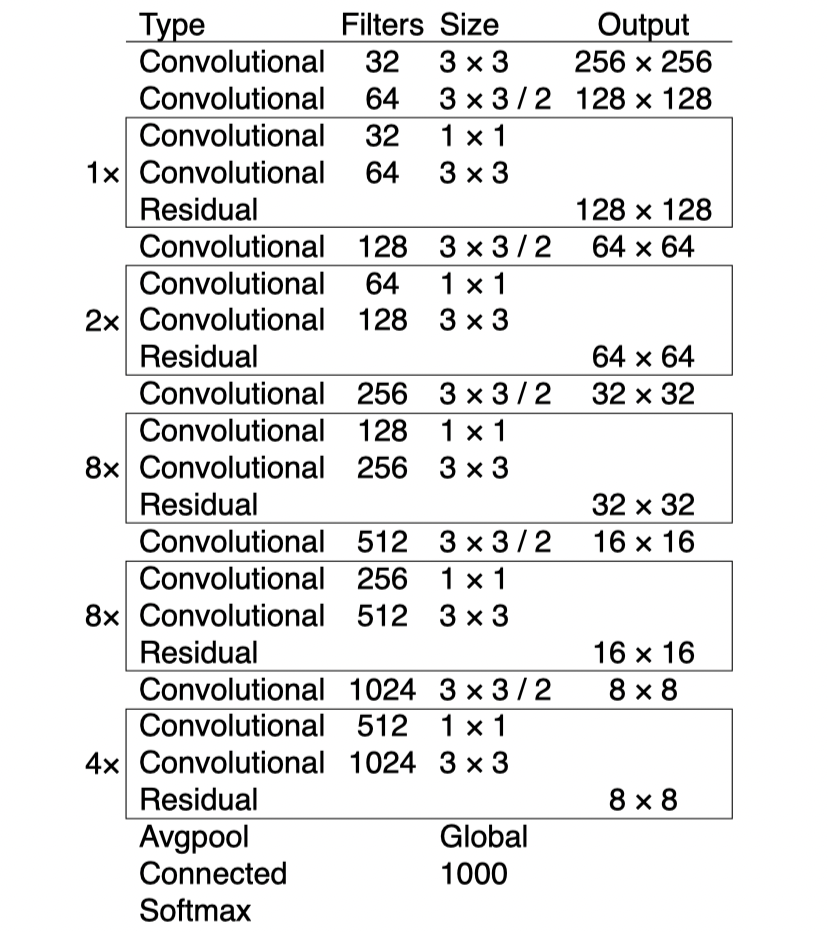
\includegraphics[width=3in]{figures/darknet53_archite.png}
    \caption{Darknet-53 architecture \cite{yolov3_2018}} 
    \label{fig:darknet53_archite}
\end{figure}